\section{Introduction}
\label{sec:introduction}

In this laboratory assignment it will be analysed a circuit composed by four
elementary meshes. The circuit includes seven resistors $R_i$, a voltage source
$V_s$, a current controlled voltage source $V_d$, a voltage controlled current
source $I_b$ and a capacitor $C$. The circuit described is portrayed in
Figure-\ref{fig:circuit}.

Throughout the report it is presented a theoretical analysis, a simulation of the
circuit and its analysis as well as a comparison of the obtained results. \par
In Section~\ref{sec:analysis}, it is applyed the nodes methods for t$<$0 and $V_s$=0,
it is determined the natural, forced ad total solutions for voltage $v_6$, such as
the frequency responses for $v_s$, $v_c$ and $v_6$, in order to do a theoretical
analysis of the circuit, using the Octave maths tool.
In Section~\ref{sec:simulation}, it is executed an analysis of the circuit using
the Ngspice tool to simulate it. In this section it is presented a simulation of
the operating point for t<0 and for $v_s$=0, the natural and total responses on node 6
and the frequency response in the same node.
In Sectione~\ref{sec:comparison}, reults obtained with both Octave and Ngspice are
displayed side-by-side, in order to compare the results.
Lastly, in Section~\ref{sec:conclusion}, it is performed a conclusion, bearing in mind the
results from both the theoretical analysis and the simulation, from Section~\ref{sec:analysis}
and Section~\ref{sec:simulation}, respectively.


\begin{figure}[h] \centering
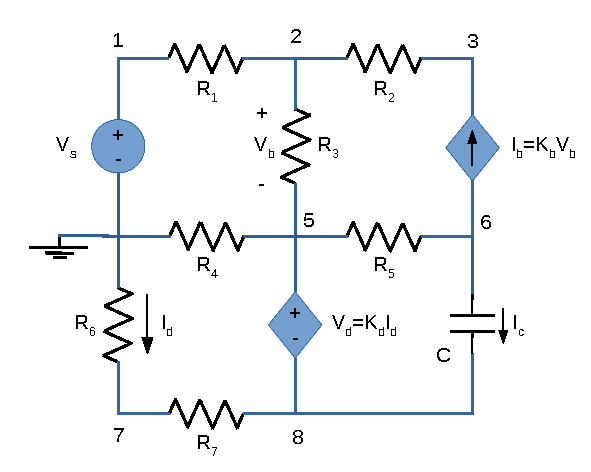
\includegraphics[width=0.7\linewidth]{circuit.pdf}
\caption{Circuit}
\label{fig:circuit}
\end{figure}

\newpage
